\documentclass{beamer}
% Configuración de la presentación
\usetheme{Hannover}
\usecolortheme{dolphin}

% Paquetes necesarios
\usepackage{graphicx}
\usepackage{amsmath}
\usepackage{url}
\usepackage{tikz}
\usetikzlibrary{shapes.geometric, arrows}
\usetikzlibrary{calc}

% Título de la presentación
\title{Documentación}
\subtitle{Proyecto: Moogle}

% Autor y afiliación
\author{Francisco Préstamo}
\institute{Universidad de la Habana}

% Fecha de la presentación
\date{2023}

\begin{document}

% Página de título
\begin{frame}
  \titlepage
\end{frame}


\begin{frame}
\frametitle{Moogle}

\begin{center}
\begin{tikzpicture}

\node (moogle) at (0,0) {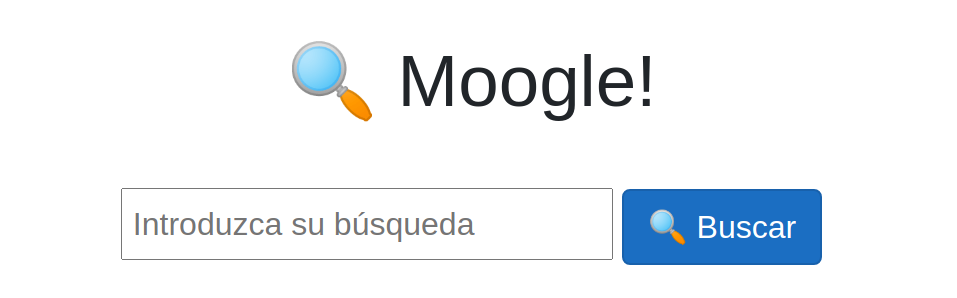
\includegraphics[width=5cm]{moogle.png}};
\draw [ultra thick, white] ($(moogle.south west) + (0.2,0.2)$) rectangle ($(moogle.north east) - (0.2,0.2)$);
\node (caption) at (0,-3) {\large Una imagen del buscador Moogle};
%\draw [->, line width=0.5mm, blue] ($(caption.north) + (0,0.2)$) -- ($(moogle.south) + (0,-0.2)$);

\end{tikzpicture}
\end{center}

\end{frame}

% Índice
\begin{frame}{Índice}
  \tableofcontents
\end{frame}

% Sección 1: Proceso de búsqueda
\section{Proceso de búsqueda}

\begin{frame}{Proceso de búsqueda}
  \begin{enumerate}
    \item El usuario ingresa una consulta en formato de texto.
    \item El buscador procesa la consulta y la transforma en un vector de términos.
    \item El buscador calcula el peso de cada término en el vector utilizando la medida tf-idf.
    \item El buscador utiliza la medida de similitud del coseno para comparar el vector de la consulta con los vectores de los documentos almacenados.
    \item Los documentos más similares se devuelven al usuario como resultados de búsqueda.
  \end{enumerate}
\end{frame}

% Sección 2: Herramientas utilizadas
\section{Herramientas utilizadas}

\begin{frame}{Herramientas utilizadas}
  \begin{itemize}
    \item \textbf{tf-idf}: medida de importancia de un término en un documento.
    \item \textbf{Similaridad del coseno}: medida de similitud entre dos vectores.
    \item \textbf{Distancia de Levenshtein}: medida de distancia entre dos cadenas de caracteres.
    \item \textbf{Operadores de búsqueda}: \texttt{!} (negación), \texttt{\^{}} (exponenciación), \texttt{*} (comodín) y \texttt{\~{}} (proximidad).
  \end{itemize}
\end{frame}

% Sección 3: Proceso de creación del buscador
\section{Proceso de creación del buscador}

\begin{frame}{Proceso de creación del buscador}
  \begin{itemize}
    \item En un principio, el buscador utilizaba arrays unidimensionales y bidimensionales para guardar la información de los documentos.
    \item Posteriormente, se implementó el uso de un array de diccionarios que permitió una mejor organización y acceso a la información de los documentos todo esto mediante una abstraccion en una clase matriz.
    \item Se agregó el uso de la distancia de Levenshtein para acercar la consulta a las palabras más parecidas dentro del universo de palabras.
    \item Se implementó la carga de información en tiempo real para que el buscador pudiera detectar y manejar los documentos que se agregan, editan o eliminan mientras el buscador está en ejecución.
  \end{itemize}
\end{frame}

% Sección 4: Gráfico
\section{Gráficos}

\begin{frame}{Gráfico}
    \frametitle{Identificación de cambios en la carpeta de documentos}

    \begin{center}
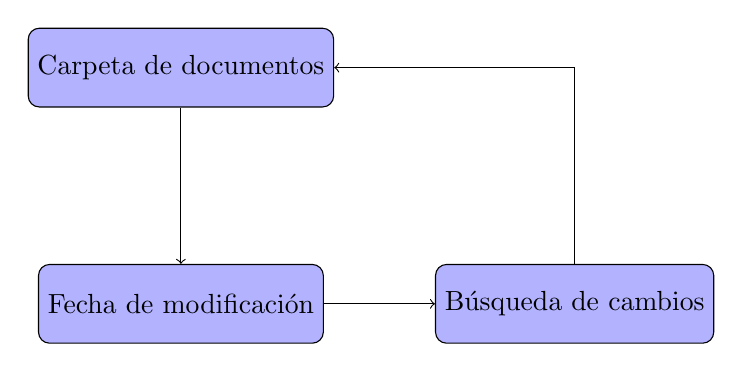
\begin{tikzpicture}[node distance=2cm, every node/.style={fill=blue!30, rounded corners, minimum width=2.5cm, minimum height=1cm, text centered, draw=black}]

\node (docs) {Carpeta de documentos};
\node (moddate) [below of=docs, yshift=-1cm] {Fecha de modificación};
\node (search) [right of=moddate, xshift=3cm] {Búsqueda de cambios};

\draw [->] (docs) -- (moddate);
\draw [->] (moddate) -- (search);
\draw [->] (search) |- (docs);

\end{tikzpicture}
\end{center}

\begin{itemize}
\item La carpeta de documentos contiene los archivos que el buscador indexa.
\item La fecha de modificación se utiliza para identificar cambios en la carpeta.
\item La búsqueda de cambios se encarga de comparar las fechas para identificar si se han producido cambios.
\end{itemize}
    
\end{frame}

% Página de agradecimientos
\begin{frame}{¡Gracias por su atención!}
  \begin{center}
    \Large ¿Preguntas?
  \end{center}
\end{frame}

\end{document}  

\usepackage{tikz}
\usetikzlibrary{shapes.geometric, arrows}
\usetikzlibrary{calc}

% Título de la presentación
\title{Documentación}
\subtitle{Proyecto: Moogle}

% Autor y afiliación
\author{Francisco Préstamo}
\institute{Universidad de la Habana}

% Fecha de la presentación
\date{2023}

\begin{document}

% Página de título
\begin{frame}
  \titlepage
\end{frame}


\begin{frame}
\frametitle{Moogle}

\begin{center}
\begin{tikzpicture}

\node (moogle) at (0,0) {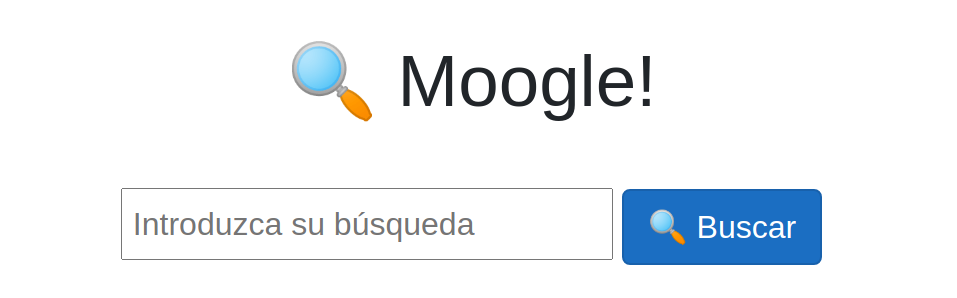
\includegraphics[width=5cm]{moogle.png}};
\draw [ultra thick, white] ($(moogle.south west) + (0.2,0.2)$) rectangle ($(moogle.north east) - (0.2,0.2)$);
\node (caption) at (0,-3) {\large Una imagen del buscador Moogle};
%\draw [->, line width=0.5mm, blue] ($(caption.north) + (0,0.2)$) -- ($(moogle.south) + (0,-0.2)$);

\end{tikzpicture}
\end{center}

\end{frame}

% Índice
\begin{frame}{Índice}
	\tableofcontents
\end{frame}

% Sección 1: Proceso de búsqueda
\section{Proceso de búsqueda}

\begin{frame}{Proceso de búsqueda}
  \begin{enumerate}
    \item El usuario ingresa una consulta en formato de texto.
    \item El buscador procesa la consulta y la transforma en un vector de términos.
    \item El buscador calcula el peso de cada término en el vector utilizando la medida tf-idf.
    \item El buscador utiliza la medida de similitud del coseno para comparar el vector de la consulta con los vectores de los documentos almacenados.
    \item Los documentos más similares se devuelven al usuario como resultados de búsqueda.
  \end{enumerate}
\end{frame}

% Sección 2: Herramientas utilizadas
\section{Herramientas utilizadas}

\begin{frame}{Herramientas utilizadas}
  \begin{itemize}
    \item \textbf{tf-idf}: medida de importancia de un término en un documento.
    \item \textbf{Similaridad del coseno}: medida de similitud entre dos vectores.
    \item \textbf{Distancia de Levenshtein}: medida de distancia entre dos cadenas de caracteres.
    \item \textbf{Operadores de búsqueda}: \texttt{!} (negación), \texttt{\^{}} (exponenciación), \texttt{*} (comodín) y \texttt{\~{}} (proximidad).
  \end{itemize}
\end{frame}

% Sección 3: Proceso de creación del buscador
\section{Proceso de creación del buscador}

\begin{frame}{Proceso de creación del buscador}
  \begin{itemize}
    \item En un principio, el buscador utilizaba arrays unidimensionales y bidimensionales para guardar la información de los documentos.
    \item Posteriormente, se implementó el uso de un array de diccionarios que permitió una mejor organización y acceso a la información de los documentos todo esto mediante una abstraccion en una clase matriz.
    \item Se agregó el uso de la distancia de Levenshtein para acercar la consulta a las palabras más parecidas dentro del universo de palabras.
    \item Se implementó la carga de información en tiempo real para que el buscador pudiera detectar y manejar los documentos que se agregan, editan o eliminan mientras el buscador está en ejecución.
  \end{itemize}
\end{frame}

% Sección 4: Gráfico
\section{Gráficos}

\begin{frame}{Gráfico}
    \frametitle{Identificación de cambios en la carpeta de documentos}

    \begin{center}
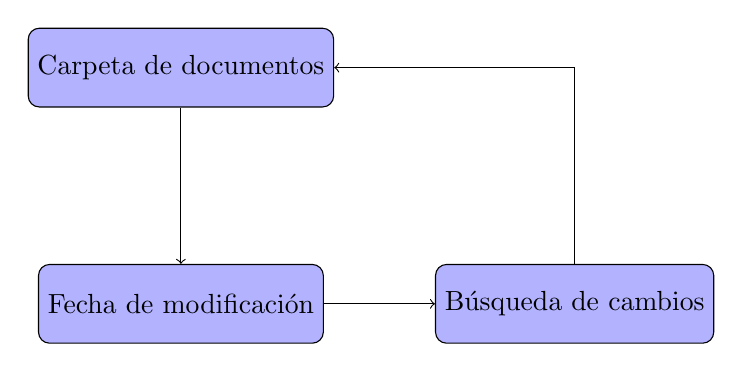
\begin{tikzpicture}[node distance=2cm, every node/.style={fill=blue!30, rounded corners, minimum width=2.5cm, minimum height=1cm, text centered, draw=black}]

\node (docs) {Carpeta de documentos};
\node (moddate) [below of=docs, yshift=-1cm] {Fecha de modificación};
\node (search) [right of=moddate, xshift=3cm] {Búsqueda de cambios};

\draw [->] (docs) -- (moddate);
\draw [->] (moddate) -- (search);
\draw [->] (search) |- (docs);

\end{tikzpicture}
\end{center}

\begin{itemize}
\item La carpeta de documentos contiene los archivos que el buscador indexa.
\item La fecha de modificación se utiliza para identificar cambios en la carpeta.
\item La búsqueda de cambios se encarga de comparar las fechas para identificar si se han producido cambios.
\end{itemize}
    
\end{frame}

% Página de agradecimientos
\begin{frame}{¡Gracias por su atención!}
  \begin{center}
    \Large ¿Preguntas?
  \end{center}
\end{frame}

\end{document}  
